\chapter{Ergebnisse}
\label{sec:ergebnisse}

\section{Versuchsteil 1: }
Die Auswertung des ersten Teilversuchs beläuft sich auf die Berechnung der jeweiligen Rohrreibungszahlen $\lambda$ für die verschiedenen Rohre unterschiedlicher hydraulischer Glattheit. Dazu müssen zuerst die Volumenströme mittels der gemessenen Wasservolumina und Durchlaufzeiten und damit die mittleren Strömungsgeschwindigkeiten berechnet werden. Im Folgenden sind dazu beispielhaft Berechnungen aufgezeigt. \\ 
Die jeweiligen Druckverluste für jede Messung ergeben sich aus der Differenz der angezeigten Manometerdrücke am Anfang und am Ende der zu untersuchenden Rohrleitungen. \\
Die berechneten Volumenströme, Geschwindigkeiten und Druckverluste sind die Grundlage für weiterführende Berechnungen hinsichtlich Reynoldszahl $Re$ und Rohrreibungszahl $\lambda$, sowie deren grafische Auswertung im Moody-Diagramm \linebreak (siehe Anhang).\\
Mit der kinetischen Viskosität können folglich die jeweiligen Reynoldszahlen berechnet werden. Beispielhaft wird die Rechnung für das hydraulisch raue Rohr gezeigt.\\
Die einzelnen Rohrleitungswiderstände für die zu untersuchenden Rohre berechnen sich nach der folgenden Formel und sind vollständig in Tab. \ref{tab:berechnung3} für alle drei Rohrleitungen aufgeführt.\\ 

\textcolor{red}{Tabellen aufsteigend sortiert nach Druckverlustwerten}

%Tabelle START
\renewcommand{\arraystretch}{1.2}
\begin{table}[h!]
	\centering
	\caption{Messwerte zu Volumen, Zeit und Druck}
	\label{tab:messwerte}
	\makebox[\textwidth]{
	\resizebox{14cm}{!}{
		\begin{tabular}{c|c|c|c|c}
			\textbf{Messpunkt}	& \textbf{Volumen $\boldsymbol{\left[\si{\raiseto{3}\meter}\right]}$} & \textbf{Zeit $\boldsymbol{\left[\si{\second}\right]}$} &\textbf{Druck 1 $\boldsymbol{\left[\si{\bar}\right]}$}	& \textbf{Druck 2 $\boldsymbol{\left[\si{\bar}\right]}$} \\
			\hline
			\multicolumn{5}{l}{raues Rohr} \\
			\hline
			1&0,01&37,6&0,07&0,01\\
			2&0,01&25,2&0,18&0,04\\
			3&0,01&18,4&0,35&0,10\\
			4&0,01&16,8&0,45&0,14\\
			5&0,01&14,9&0,56&0,17\\
			\hline
			\multicolumn{5}{l}{glattes Rohr} \\
			\hline
			1&0,01&17,1&0,28&0,05\\
			2&0,01&15,0&0,36&0,06\\
			(3)&(0,01)&(12,3)&(0,44)&(0,10)\\
			4&0,01&13,5&0,43&0,07\\
			5&0,01&12,6&0,49&0,09\\
			\hline
			\multicolumn{5}{l}{glattes, dickes Rohr} \\
			\hline
			1&0,01&10,6&0,11&0,04\\
			2&0,01&9,1&0,15&0,07\\
			3&0,01&7,9&0,23&0,10\\
			4&0,01&7,3&0,26&0,12\\
			5&0,01&6,5&0,33&0,16\\
			\hline
		\end{tabular}}}
\end{table}
\FloatBarrier
\vspace*{-2.5mm}
%Tabelle Ende

\subsection*{Berechnung des Volumenstroms}
\begin{flalign}
	\dot{V}	&= \frac{V}{t}\\[2mm]
	\dot{V}_{1,rau}	&= \frac{V_{1,rau}}{t_{1,rau}}	\\
				&= \frac{\SI{0,01}{\raiseto{3} \meter}}{\SI{37,6}{\second}}\\
				&= \SI{2,66e-4}{\raiseto{3} \meter\per\second} \approx \underline{\underline{\SI{958}{\liter\per\hour}}}
\end{flalign}
\subsection*{Berechnung der mittleren Geschwindigkeit}
\begin{flalign}
\overline{\omega}	&= \frac{\dot{V}}{A}\\[1mm]
					&=\frac{4*\dot{V}}{\pi*d^2}\\[1mm]
\overline{\omega}_{1,rau}	&=\frac{4*\dot{V}_{1,rau}}{\pi*\left(d_{1,rau}\right)^2}\\
							&= \frac{4*\SI{2,66e-4}{\raiseto{3} \meter\per\second}}{\pi*\left(\SI{13,6e-3}{\meter}\right)^2}\\
							&=\underline{\underline{\SI{1,83}{\meter \per\second}}}
\end{flalign}
\subsection*{Berechnung des Druckverlustes}
\begin{flalign}
	\Delta p_v		&= p_{i,rau,1}-p_{i,rau,2}\\
	\Delta p_{v_{1,rau}} &= p_{1,rau,1}-p_{1,rau,2}\\
					&= \SI{0,07}{\bar}-\SI{0,01}{\bar}\\
					&=\underline{\underline{\SI{0,06}{\bar}}} \quad (\SI{0,056}{\bar})
\end{flalign}
%Tabelle START
\vspace*{-7.5mm}
\renewcommand{\arraystretch}{1.2}
\begin{table}[h!]
	\centering
	\caption{Volumenströme, mittlere Geschwindigkeiten und Druckverluste}
	\label{tab:berechnung1}
	\makebox[\textwidth]{
	\resizebox{17cm}{!}{
		\begin{tabular}{c|c|c|c}
			\textbf{Messpunkt}	& \textbf{Volumenstrom $\boldsymbol{\left[\si{\liter\per\minute}\right]}$} & \textbf{mittlere Geschwindigkeit $\boldsymbol{\left[\si{\meter \per \second}\right]}$}	& \textbf{Druckverlust $\boldsymbol{\left[\si{\bar}\right]}$}\\
			\hline
			\multicolumn{4}{l}{raues Rohr} \\
			\hline
			1&958&1,83&0,06\\
			2&1430&2,73&0,14\\
			3&1962&3,75&0,25\\
			4&2139&4,09&0,32\\
			5&2413&4,61&0,39\\
			\hline
			\multicolumn{4}{l}{glattes Rohr} \\
			\hline
			1&2111&4,04&0,23\\
			2&2406&4,60&0,30\\
			(3)&(2922)&(5,59)&(0,34)\\
			4&2667&5,10&0,36\\
			5&2866&5,48&0,40\\
			\hline
			\multicolumn{4}{l}{glattes, dickes Rohr} \\
			\hline
			1&3403&2,49&0,07\\
			2&3978&2,91&0,08\\
			3&4557&3,33&0,13\\
			4&4932&3,60&0,14\\
			5&5513&4,03&0,17\\
			\hline
		\end{tabular}
	}}
\end{table}
\FloatBarrier
\vspace*{-2.5mm}
%Tabelle Ende
Die folgende Gleichung für die Dichte des Wasser stammt aus linear interpolierten Daten, welche mittels Excel-AddIn für unterschiedlichen Temperaturen bestimmt wurde (siehe \cite{BernhardSpang.2002}). Genutzt wurde dafür die Funktion \texttt{=densW(T$\left[\si{\kelvin}\right]$,p$\left[\si{\bar}\right]$)} mit der Annahme, dass der Druck konstant \SI{1}{\bar} beträgt. Analog gilt dasselbe für die dynamische Viskosität mittels der Funktion \texttt{=viscW(T$\left[\si{\kelvin}\right]$,p$\left[\si{\bar}\right]$)} mit der man in Folge die kinetische Viskosität errechnen kann. \\
In Bezug auf die Dichtefunktion wurde zwischen der maximal und minimal im Versuch gemessenen Temperatur interpoliert. Die interpolierten Werte sind der Tabelle \ref{tab:dichte} im Anhang unter Abschnitt \ref{sec:anhang} zu entnehmen, sowie die Gleichung selbst unter Gleichung \ref{gl:dichte}.
\begin{flalign}
\label{gl:dichte}
\rho(T) &= \SI{-0,2683}{\kg \per \raiseto{3} \meter \per \kelvin} * T+\SI{1003,8}{\kg \per \raiseto{3} \meter}
\end{flalign}

\subsection*{Berechnung der kinetischen Viskosität}

\begin{flalign}
\nu	&= \frac{\eta}{\rho(T)}\\[2mm]
\nu_{1,rau}	&=\frac{\SI{8,63e-4}{\pascal\second}}{\SI{996,7}{\kg\per\raiseto{3}\meter}}\\
			&=\underline{\underline{\SI{8,66e-7}{\raiseto{2}\meter\per\second}}}
\end{flalign}
\subsection*{Berechnung der Reynoldszahl}
\begin{flalign}
Re	&=\frac{\overline{\omega}*d}{\nu}\\
Re_{1,rau}	&=\frac{\overline{\omega}_{1,rau}*d_{1,rau}}{\nu_{1,rau}}\\
			&= \frac{\SI{1,83}{\meter\per\second}*\SI{13,6e-3}{\meter}}{\SI{8,66e-7}{\raiseto{2}\meter\per\second}}\\
			&\approx \underline{\underline{71687}}
\end{flalign}

%Tabelle START
\vspace*{-10.5mm}
\renewcommand{\arraystretch}{1.2}
\begin{table}[h!]
	\centering
	\caption{Temperaturen, Dichten, kinetische Viskositäten und Reynoldszahlen}
	\label{tab:berechnung2}
	%\resizebox{12.6cm}{!}{
	\begin{tabular}{c|c|c|c|c}
		\textbf{Messpunkt}	& \textbf{Temperatur} & \textbf{Dichte}	& \textbf{kine. Viskosität $\left[10^{-7}\right]$} & \textbf{Reynoldszahl}\\
		\hline
		\multicolumn{5}{l}{raues Rohr} \\
		\hline
		1&26,5&996,7&8,66&28766\\
		2&26,8&996,6&8,61&43206\\
		3&27,3&996,5&8,51&59940\\
		4&27,5&996,4&8,47&65639\\
		5&26,3&996,7&8,70&72117\\
		\hline
		\multicolumn{5}{l}{glattes Rohr} \\
		\hline
		1&26,3&996,7&8,70&63108\\
		2&26,1&996,8&8,74&71606\\
		(3)&(25,4)&(997,0)&(8,88)&(85602)\\
		4&25,9&996,9&8,78&78998\\
		5&25,6&996,9&8,84&84344\\
		\hline
		\multicolumn{5}{l}{glattes, dickes Rohr} \\
		\hline
		1&27,3&996,5&8,51&64267\\
		2&27,0&996,6&8,57&74640\\
		3&26,9&996,6&8,59&85318\\
		4&26,6&996,7&8,64&91723\\
		5&26,3&996,7&8,70&101862\\
		\hline
	\end{tabular}
	%	}
\end{table}
\FloatBarrier
\vspace*{-2.5mm}
%Tabelle Ende
\subsection*{Berechnung des Rohrleitungswiderstandes}
\begin{flalign}
\lambda &= \frac{2*\Delta p_v*d}{l*\rho(T)*v^2}\\[2mm]
\lambda_{1,rau} &= \frac{2*\Delta p_{v_{1,rau}}*d}{l_{1,rau}*\rho(T)_{1,rau}*\left(v_{1,rau}\right)^2}\\
				&= \frac{2*\SI{5600}{\pascal}*\SI{13,6e-3}{\meter}}{\SI{2,5}{\meter}*\SI{996,7}{\kg\per\raiseto{3}\meter}*\left(\SI{1,83}{\meter\per\second}\right)^2}\\
				&= \underline{\underline{0,018}}
\end{flalign}

%Tabelle START
\vspace*{-10.5mm}
\renewcommand{\arraystretch}{1.2}
\begin{table}[h!]
	\centering
	\caption{Druckverluste, Volumenströme und Rohrleitungswiderstände}
	\label{tab:berechnung3}
	%\resizebox{12.6cm}{!}{
	\begin{tabular}{c|c|c|c}
		\textbf{Messpunkt}	& \textbf{Volumenstrom} &\textbf{Druckverlust}	& \textbf{Rohrleitungswiderstand} \\
		\hline
		\multicolumn{4}{l}{raues Rohr} \\
		\hline
		1&958&0,06&0,018\\
		2&1430&0,14&0,020\\
		3&1962&0,25&0,019\\
		4&2139&0,32&0,021\\
		5&2413&0,41&0,020\\
		\hline
		\multicolumn{4}{l}{glattes Rohr} \\
		\hline
		1&2111&0,24&0,026\\
		2&2406&0,30&0,026\\
		(3)&(2922)&(0,034)&(0,020)\\
		4&2667&0,36&0,025\\
		5&2866&0,41&0,025\\
		\hline
		\multicolumn{4}{l}{glattes, dickes Rohr} \\
		\hline
		1&3403&0,07&0,031\\
		2&3978&0,08&0,029\\
		3&4557&0,13&0,033\\
		4&4932&0,14&0,031\\
		5&5513&0,17&0,031\\
		\hline
	\end{tabular}
	%	}
\end{table}
\FloatBarrier
\vspace*{-2.5mm}
%Tabelle Ende

%Tabelle START
\vspace*{-5.5mm}
\renewcommand{\arraystretch}{1.2}
\begin{table}[h!]
	\centering
	\caption{Mittelwerte der Rohrleitungswiderstände}
	\label{tab:l_mittel}
	%\resizebox{12.6cm}{!}{
	\begin{tabular}{c|c}
		\textbf{Rohr}	& \textbf{Mittlerer Rohrleitungswiderstand}  \\
		\hline
		raues Rohr & 0.0196\\
		glattes Rohr & 0.0254\\
		glattes, dickes Rohr &0.0309\\
		\hline
	\end{tabular}
	%	}
\end{table}
\FloatBarrier
%Tabelle Ende
\vspace*{-2.5mm}
% pgf diagramm3 START
\begin{figure}[h!]
	\begin{center}
		%\resizebox{0.8\textwidth}{!}{
		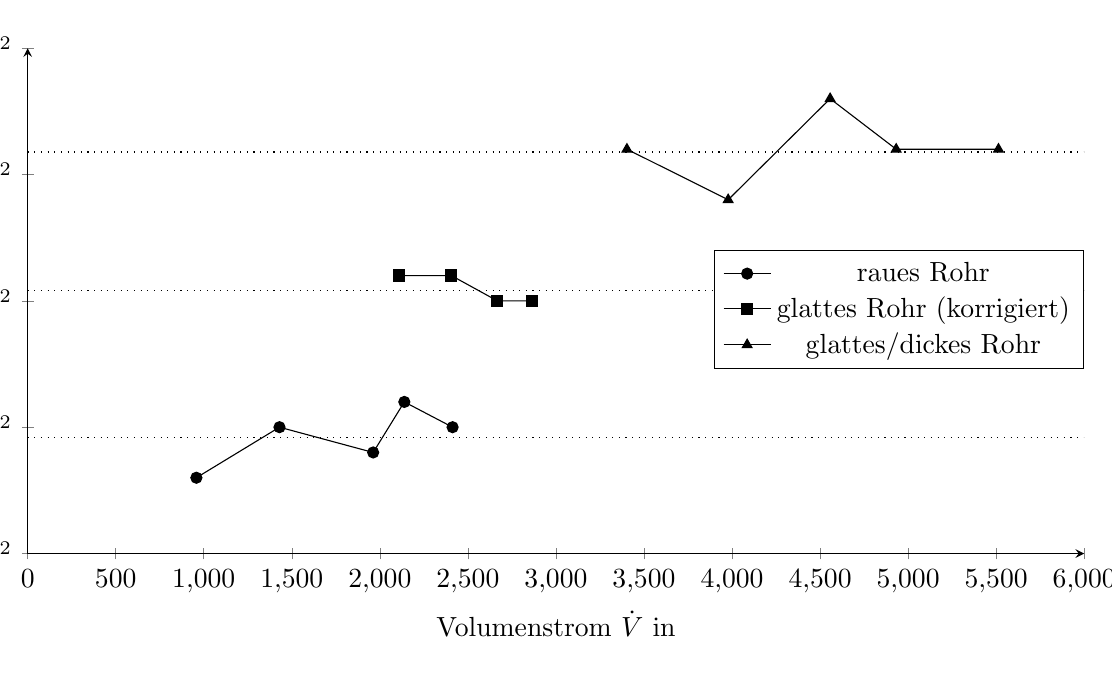
\begin{tikzpicture}[trim axis left, trim axis right]
		\begin{axis}[
		axis lines = left,
		width = 15cm,
		height = 8cm,
		xmin = 0,
		xmax = 6000,
		ymin = 0.015,
		ymax = 0.035,
		ylabel={Rohrleitungswiderstand $\lambda$},
		y label style={at={(-0.095,0.5)}},
		xlabel={Volumenstrom $\dot{V}$ in \si{\liter \per \minute}},
		scaled ticks=false ,
		legend style={at={(1.,0.6)}}
		]
		%rau
		\addplot[black,mark=*,text mark as node=true,point meta=explicit symbolic,nodes near coords]
		coordinates {(958,0.018) (1430,0.02) (1962,0.019) (2139,0.021) (2413,0.020)};
		
		%glatt (korrigiert)
		\addplot[black,mark=square*,text mark as node=true,point meta=explicit symbolic,nodes near coords]
		coordinates {(2111,0.026) (2406,0.026) (2667,0.025) (2866,0.025)};
		
		
		%glatt, dickes Rohr
		\addplot[black,mark=triangle*,text mark as node=true,point meta=explicit symbolic,nodes near coords]
		coordinates {(3403,0.031) (3978,0.029) (4557,0.033) (4932,0.031) (5513,0.031)};
		
		%Mittelwerte
		\addplot[no markers, dotted] coordinates {(0,0.0196)(6000,0.0196)};
		\addplot[no markers, dotted] coordinates {(0,0.0254)(6000,0.0254)};
		\addplot[no markers, dotted] coordinates {(0,0.03089)(6000,0.03089)};
		
		\legend{raues Rohr, glattes Rohr (korrigiert), glattes/dickes Rohr}
		\end{axis}
		\end{tikzpicture}
		%	}
		\caption{Druckverlust in Abhängigkeit zum Volumenstrom}
		\label{dia:lzuv}
	\end{center}
\end{figure}
\FloatBarrier

\vspace*{-2.5mm}
% pgf diagramm3 START
\begin{figure}[h!]
	\begin{center}
		%\resizebox{0.8\textwidth}{!}{
		\begin{tikzpicture}[trim axis left, trim axis right]
		\begin{axis}[
		axis lines = left,
		width = 13cm,
		height = 7.5cm,
		xmin = 0,
		xmax = 0.45,
		ymin = 0.015,
		ymax = 0.035,
		ylabel={Rohrleitungswiderstand $\lambda$},
		y label style={at={(-0.095,0.5)}},
		xlabel={Druckverlust $\Delta p_V$ in \si{\bar}},
		scaled ticks=false ,
		legend style={at={(1.3,1.1)}}
		]
		%rau
		\addplot[black,mark=*,text mark as node=true,point meta=explicit symbolic,nodes near coords]
		coordinates {(0.056,0.018) (0.14,0.02) (0.25,0.019) (0.315,0.021) (0.382,0.02)};

		%glatt (korrigiert)
		\addplot[black,mark=square*,text mark as node=true,point meta=explicit symbolic,nodes near coords]
		coordinates {(0.235,0.026) (0.3,0.026) (0.358,0.025) (0.405,0.025)};
		
		
		%glatt, dickes Rohr
		\addplot[black,mark=triangle*,text mark as node=true,point meta=explicit symbolic,nodes near coords]
		coordinates {(0.065,0.0309) (0.083,0.0289) (0.125,0.0332) (0.135,0.0306) (0.17,0.0308)};
		
		%Mittelwerte
		\addplot[no markers, dotted] coordinates {(0,0.0196)(0.5,0.0196)};
		\addplot[no markers, dotted] coordinates {(0,0.0254)(0.5,0.0254)};
		\addplot[no markers, dotted] coordinates {(0,0.03089)(0.5,0.03089)};
		
		\legend{raues Rohr, glattes Rohr (korrigiert), glattes/dickes Rohr, Mittelwerte $\lambda$}
		\end{axis}
		\end{tikzpicture}
		%	}
		\caption{$\lambda$ zu Druckverlust }
		\label{dia:lzud}
	\end{center}
\end{figure}
\FloatBarrier

\vspace*{-2.5mm}
% pgf diagramm3 START
\begin{figure}[h!]
	\begin{center}
		%\resizebox{0.8\textwidth}{!}{
		\begin{tikzpicture}[trim axis left, trim axis right]
		\begin{axis}[
		axis lines = left,
		width = 15cm,
		height = 8cm,
		xmin = 0,
		xmax = 6000,
		ymin = 0,
		ymax = 0.5,
		ylabel={Druckverlust $\Delta p_V$ in \si{\bar}},
		y label style={at={(-0.,0.5)}},
		xlabel={Volumenstrom $\dot{V}$ in \si{\liter \per \minute}},
		scaled ticks=false ,
		legend style={at={(1,1)}}
		]
		%rau
		\addplot[black,mark=*,text mark as node=true,point meta=explicit symbolic,nodes near coords]
		coordinates {(958,0.056) (1430,0.14) (1962,0.25) (2139,0.315) (2413,0.382)};
		
		%glatt (korrigiert)
		\addplot[black,mark=square*,text mark as node=true,point meta=explicit symbolic,nodes near coords]
		coordinates {(2111,0.235) (2406,0.3) (2667,0.358) (2866,0.405)};
		
		
		%glatt, dickes Rohr
		\addplot[black,mark=triangle*,text mark as node=true,point meta=explicit symbolic,nodes near coords]
		coordinates {(3403,0.065) (3978,0.083) (4557,0.125) (4932,0.135) (5513,0.17)};
		
		%Trendlinien
		
		\legend{raues Rohr, glattes Rohr (korrigiert), glattes/dickes Rohr}
		\end{axis}
		\end{tikzpicture}
		%	}
		\caption{Druckverlust in Abhängigkeit zum Volumenstrom}
		\label{dia:pzuv}
	\end{center}
\end{figure}
\FloatBarrier

\textcolor{red}{Glatte Rohre müssten weniger Rohrleitungswiderastand haben, da sich aber Dichte des Wasser verringert und Volumenstrom sehr hoch ist, steigt somit laut Gleichung der Rohrleitungswiderstand}

\newpage

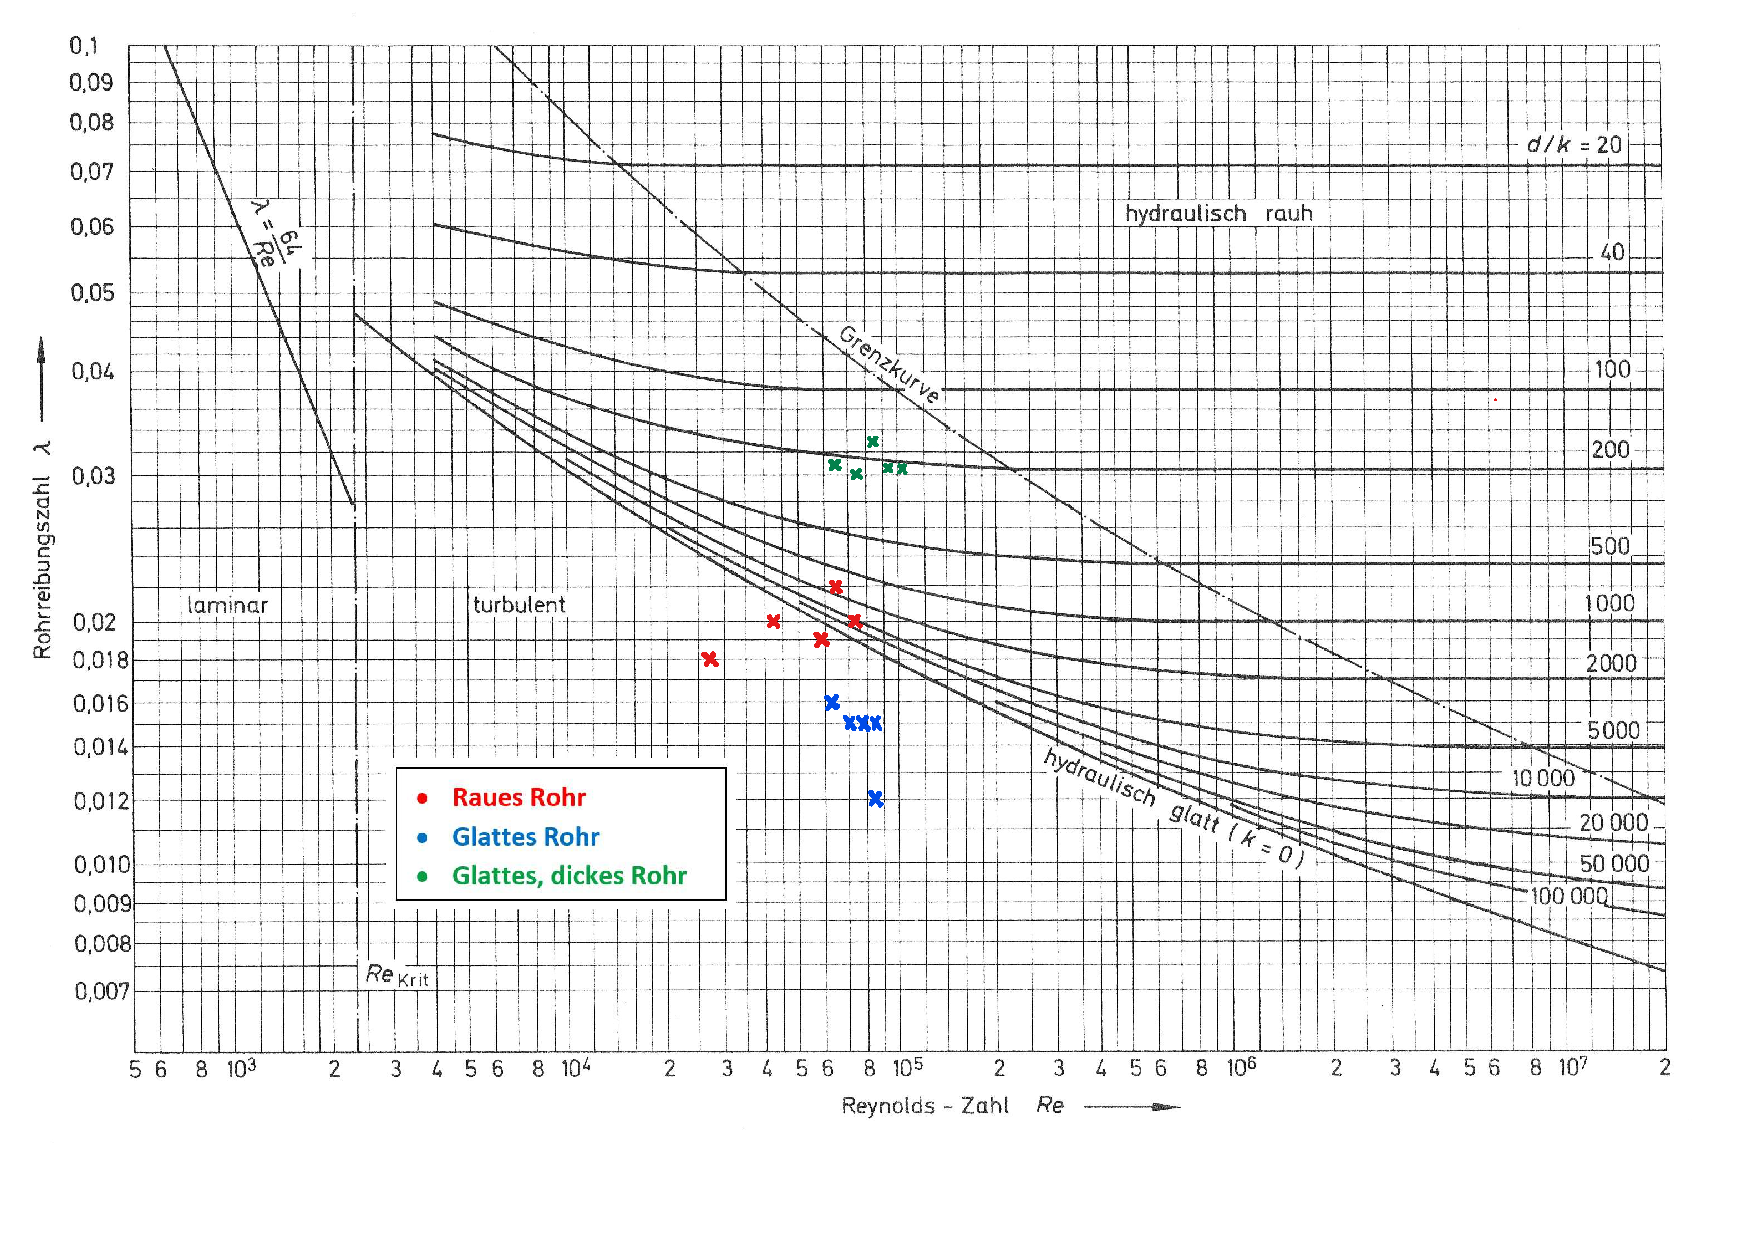
\includepdf[landscape=true,page=1]{img/Diagramm_Rohrreibungszahl2.pdf}

\newpage

\section{Versuchsteil 2:}


%Tabelle START
\vspace*{-5.5mm}
\renewcommand{\arraystretch}{1.2}
\begin{table}[h!]
	\centering
	\caption{Grundlegende Daten Schrägventil und Muffenschieber}
	\label{tab:grundlegendes}
	%\resizebox{12.6cm}{!}{
	\begin{tabular}{c|c|c|c}
		\textbf{Ventil} &\textbf{Rohrdurchmesser}	& \textbf{Volumenstrom} &\textbf{Geschwindigkeit}	 \\
		\hline
		Schrägventil& \SI{40}{\milli \meter} & \SI{47}{\liter\per\minute} & \SI{0,62}{\meter \per \second}\\
		Muffenschieber& \SI{40}{\milli \meter} & \SI{47}{\liter\per\minute} & \SI{0,62}{\meter \per \second}\\
		\hline
	\end{tabular}
	%	}
\end{table}
\FloatBarrier
\vspace*{-2.5mm}
%Tabelle Ende

%Tabelle START
\vspace*{-5.5mm}
\renewcommand{\arraystretch}{1.2}
\begin{table}[h!]
	\centering
	\caption{Messwerte Schrägventil}
	\label{tab:schragventil}
	\makebox[\textwidth]{
	\begin{tabular}{c|c|c|c|c}
		\textbf{Temperatur}&\textbf{Umdrehungen} &\textbf{Ventilhubstellung}	& \textbf{Druck 1} &\textbf{Druck 2}	 \\
		\hline
		27,3 &0&\quad \SI{0}{\degrees} | \SI{100}{\percent}&0,015&0,007\\
		27,5&1&\SI{360}{\degrees}  | \SI{98}{\percent}&0,015&0,008\\
		27,9&2&\SI{720}{\degrees}  | \SI{96}{\percent}&0,015&0,009\\
		28,2&3&\SI{1080}{\degrees} | \SI{91}{\percent}&0,015&0,009\\
		28,5&4&\SI{1440}{\degrees} | \SI{87}{\percent}&0,015&0,009\\
		28,7&5&\SI{1800}{\degrees} | \SI{78}{\percent}&0,018&0,009\\
		28,7&6&\SI{2160}{\degrees} | \SI{70}{\percent}&0,0,018&0,009\\
		28,8&7&\SI{2520}{\degrees} | \SI{61}{\percent}&0,020&0,008\\
		28,9&8&\SI{2880}{\degrees} | \SI{52}{\percent}&0,020&0,007\\
		29,0&9&\SI{3240}{\degrees} | \SI{43}{\percent}&0,025&0,005\\
		29,1&10&\SI{3600}{\degrees} | \SI{35}{\percent}&0,040&0,008\\
		29,4&10,5&\SI{3780}{\degrees} | \SI{26}{\percent}&0,070&0,008\\
		29,7&11&\SI{3960}{\degrees} | \SI{17}{\percent}&0,175&0,008\\
		29,8&11,25&\SI{4050}{\degrees} | \SI{9}{\percent}&0,460&0,009\\
		29,8&11,5&\SI{4140}{\degrees} | \SI{0}{\percent}&1,100&0,008\\
		\hline
	\end{tabular}}
\end{table}
\FloatBarrier
\vspace*{-2.5mm}
%Tabelle Ende

%Tabelle START
\vspace*{-5.5mm}
\renewcommand{\arraystretch}{1.2}
\begin{table}[h!]
	\centering
	\caption{Messwerte Muffenschieber}
	\label{tab:muffenschieber}
	\makebox[\textwidth]{
		\begin{tabular}{c|c|c|c|c}
			\textbf{Temperatur}&\textbf{Umdrehungen} &\textbf{Ventilhubstellung}	& \textbf{Druck 1} &\textbf{Druck 2}	 \\
			\hline
			29,8 &0&\quad \SI{0}{\degrees} | \SI{100}{\percent}&0,015&0,015\\
			29,9&1&\SI{360}{\degrees} | \SI{96}{\percent}&0,018&0,016\\
			29,9&2&\SI{720}{\degrees} | \SI{93}{\percent}&0,020&0,017\\
			30,0&3&\SI{1080}{\degrees} | \SI{91}{\percent}&0,025&0,017\\
			30,1&4&\SI{1440}{\degrees} | \SI{87}{\percent}&0,045&0,017\\
			30,2&5&\SI{1800}{\degrees} | \SI{70}{\percent}&0,143&0,017\\
			30,3&5,25&\SI{1890}{\degrees} | \SI{52}{\percent}&0,240&0,016\\
			30,5&5,375&\SI{1935}{\degrees} | \SI{35}{\percent}&0,435&0,017\\
			30,7&5,5&\SI{1980}{\degrees} | \SI{17}{\percent}&0,515&0,017\\
			30,8&5,75&\SI{2070}{\degrees} | \SI{0}{\percent}&1,000&0,017\\
			\hline
	\end{tabular}}
\end{table}
\FloatBarrier
\vspace*{-2.5mm}
%Tabelle Ende

\newpage

\subsection*{Berechnung des Druckverlustbeiwert}
\begin{flalign}
	\zeta	&= \frac{2*\Delta p}{\rho(T)*v^2}\\
	\zeta_{0,Schräg}	&= \frac{2*\Delta p_{0,Schräg}}{\rho(T)_{0,Schräg}*(v_{0,Schräg})^2}\\[5pt]
	&=\frac{2*\SI{800}{\pascal}}{\SI{996,5}{\kg\per\raiseto{3}\meter}*(\SI{0,62}{\meter \per \second})^2}\\
	&= \underline{\underline{4,21}}
\end{flalign}

\subsection*{Berechnung des $K_v$-Wertes}
\begin{flalign}
K_{v}			&= \dot{V}*\sqrt{\frac{\SI{1}{\bar}}{\Delta p}*\frac{\rho(T)}{\SI{1000}{\kg\per\raiseto{3}\meter}}}\\
K_{v_{0,Schräg}}&=\dot{V}_{0,Schräg}*\sqrt{\frac{\SI{1}{\bar}}{\Delta p_{0,Schräg}}*\frac{\rho(T)_{0,Schräg}}{\SI{1000}{\kg\per\raiseto{3}\meter}}}\\[4pt]
				&=\SI{47}{\liter\per\minute}*\sqrt{\frac{\SI{1}{\bar}}{\SI{0,008}{\bar}}*\frac{\SI{996,5}{\kg\per\raiseto{3}\meter}}{\SI{1000}{\kg\per\raiseto{3}\meter}}}\\
				&\approx\underline{\underline{\SI{520}{\liter\per\minute}}}
\end{flalign}

%Tabelle START
\vspace*{-5.5mm}
\renewcommand{\arraystretch}{1.2}
\begin{table}[h!]
	\centering
	\caption{Berechnete Werte Schrägventil}
	\label{tab:schragventil_ber}
	\resizebox{14cm}{!}{
	\makebox[\textwidth]{
		\begin{tabular}{c|c|c|c|c}
			\textbf{Umdrehungen}& \textbf{Dichte}& \textbf{Druckverlust}&\textbf{Druckverlustbeiwert}& \textbf{$K_v$-Wert}\\
			\hline
			0&996,5&0,008&4,2&520\\
			1&996,4&0,007&3,7&556\\
			2&996,3&0,006&3,2&600\\
			3&996,2&0,006&3,2&600\\
			4&996,1&0,006&3,2&600\\
			5&996,1&0,009&4,5&504\\
			6&996,1&0,0,009&4,7&490\\
			7&996,1&0,012&6,3&424\\
			8&996,0&0,013&6,8&408\\
			9&996,0&0,020&10,5&329\\
			10&996,0&0,032&16,8&260\\
			10,5&995,9&0,062&32,6&187\\
			11&995,8&0,167&87,9&114\\
			11,25&995,8&0,451&237,3&69\\
			11,5&995,8&1,092&574,6&45\\
			\hline
	\end{tabular}}}
\end{table}
\FloatBarrier
\vspace*{-2.5mm}
%Tabelle Ende

%Tabelle START
\vspace*{-5.5mm}
\renewcommand{\arraystretch}{1.2}
\begin{table}[h!]
	\centering
	\caption{Berechnete Werte Muffenschieber}
	\label{tab:muffenschieber_ber}
	\makebox[\textwidth]{
		\begin{tabular}{c|c|c|c|c}
			\textbf{Umdrehungen}& \textbf{Dichte}& \textbf{Druckverlust}&\textbf{Druckverlustbeiwert}& \textbf{$K_v$-Wert}\\
			\hline
			0&995,8&0,000&0&-\\
			1&995,7&0,0015&0,8&1207\\
			2&995,7&0,0030&1,6&854\\
			3&995,7&0,0080&4,2&523\\
			4&995,7&0,028&14,6&280\\
			5&995,6&0,1255&65,2&132\\
			5,25&964,6&0,0,2240&116,4&99\\
			5,375&995,5&0,4180&217,3&72\\
			5,5&995,5&0,4980&258,9&66\\
			5,75&995,5&0,9830&511,0&47\\
			\hline
	\end{tabular}}
\end{table}
\FloatBarrier
\vspace*{-2.5mm}
%Tabelle Ende


\vspace*{-2.5mm}
% pgf diagramm3 START
\begin{figure}[h!]
	\begin{center}
		%\resizebox{0.8\textwidth}{!}{
		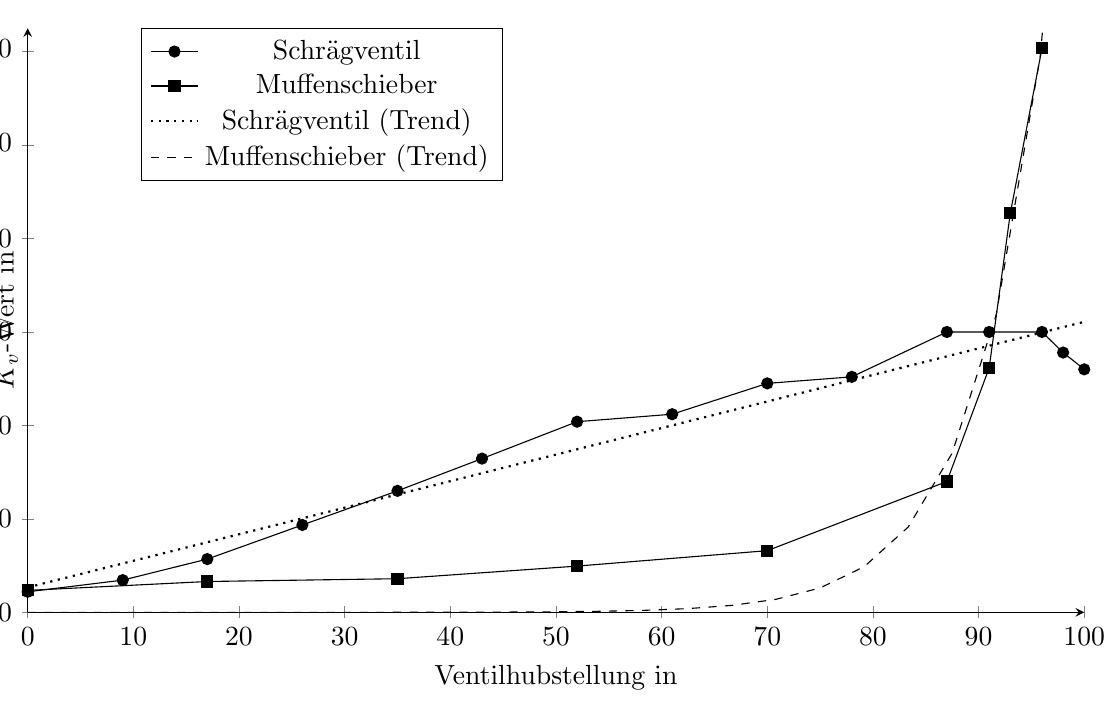
\begin{tikzpicture}[trim axis left, trim axis right]
		\begin{axis}[
		axis lines = left,
		width = 15cm,
		height = 9cm,
		xmin = 0,
		xmax = 100,
		ymin = 0,
		ymax = 1250,
		ylabel={$K_v$-Wert in \si{\liter\per\minute}},
		y label style={at={(-0.,0.5)}},
		xlabel={Ventilhubstellung in \si{\percent}},
		scaled ticks=false ,
		legend style={at={(0.45,1)}}
		]
		%schräg
		\addplot[black,mark=*,text mark as node=true,point meta=explicit symbolic,nodes near coords]
		coordinates {(100,520) (98,556) (96,600) (91,600) (87,600) (78,504) (70,490) (61,424) (52,408) (43,329) (35,260) (26,187) (17,114) (9,69) (0,44)};
		
		%Muffe
		\addplot[black,mark=square*,text mark as node=true,point meta=explicit symbolic,nodes near coords]
		coordinates {(96,1207) (93,854) (91,523) (87,280) (70,132) (52,99) (35,72) (17,66) (0,47)};
		
		\addplot[black,mark=none,text mark as node=true,point meta=explicit symbolic,nodes near coords,thick,dotted][domain=0:100]{5.6824*x + 53.456};
		
		%Trend Muffe
		\addplot[black,mark=none,text mark as node=true,point meta=explicit symbolic,nodes near coords,dashed][domain=0:100]{0.000829961*(1.161889742)^(x-1.358635786)};
		
		\legend{Schrägventil, Muffenschieber, Schrägventil (Trend) , Muffenschieber (Trend)}
		\end{axis}
		\end{tikzpicture}
		%	}
		\caption{$K_V$ in Abhängigkeit von der Ventilhubstellung}
		\label{dia:Kv}
	\end{center}
\end{figure}
\FloatBarrier

\textbf{Gleichungen für die Trendkurven:}
\begin{itemize}
	\item Schrägventil mittels linearer Regression: \\
	$f(x)=5,6824*x + 53,456$
	\item Muffenschieber mittels Wachstumsgleichung: \\
	$g(x)=0,000829961*(1,161889742)^{(x-1,358635786)}$
\end{itemize}




